\documentclass[11pt]{article}
\usepackage[review]{acl}
\usepackage{times}
\usepackage{latexsym}
\usepackage[T1]{fontenc}
\usepackage[utf8]{inputenc}
% This is not strictly necessary, and may be commented out,
% but it will improve the layout of the manuscript,
% and will typically save some space.
\usepackage{microtype}
% This is also not strictly necessary, and may be commented out.
% However, it will improve the aesthetics of text in
% the typewriter font.
\usepackage{inconsolata}
\usepackage{graphicx}

% If the title and author information does not fit in the area allocated, uncomment the following
%
%\setlength\titlebox{<dim>}
%
% and set <dim> to something 5cm or larger.

\title{The Silence of the Facts: Popularity as a Barrier to Machine Unlearning}


\author{First Author \\
  Affiliation / Address line 1 \\
  Affiliation / Address line 2 \\
  Affiliation / Address line 3 \\
  \texttt{email@domain} \\\And
  Second Author \\
  Affiliation / Address line 1 \\
  Affiliation / Address line 2 \\
  Affiliation / Address line 3 \\
  \texttt{email@domain} \\}


\begin{document}
\maketitle
\begin{abstract}
Machine Unlearning is a valuable ability of LLMs, enabling removal of unsafe, outdated, or private information. Existing unlearning methods, however, are often evaluated under the assumption that all facts are equally challenging to forget. Controllable removal of knowledge is essential for reliable NLP systems. In this paper, we are investigating whether fact popularity influence efficiency of LLM unlearning. 
%
To answer this question, we build \textit{UNLamb} benchmark designed to systematically investigate this relationship. It consists of 11.6k question-answer pairs derived from real-world knowledge in Wikidata, explicitly partitioned into rare and popular facts. Using this benchmark, we perform a comprehensive evaluation of state-of-the-art unlearning algorithms on a set of models of different sizes. 
We conduct a comprehensive analysis of four unlearning methods%: GA, GD, NPO, and RMU, 
across three validation sets and two LLMs. We show that, larger models struggle more to forget popular  entities often damaging related knowledge when trying to forget them. In contrast, it is much easier to remove rare facts without side effects. %Thus, current unlearning methods do not suffice and highlights the need for new strategies that account for the popularity of facts. %The experiments presented here provide a foundation for adapting future unlearning algorithms to incorporate fact popularity as an explicit signal, enabling more stable and predictable knowledge removal from LLMs.
%\textcolor{red}{Our findings are also relevant to the evaluation of agentic LLM systems, since controllable removal of knowledge is essential for reliable, aligned agents that operate over long horizons and evolving goals.}
\end{abstract}





\section{Introduction}
\label{sec:intro}

Large Language Models (LLMs) are backbone of the modern NLP technology, yet they  are largely trained on Web texts which often include private, copyrighted, outdated or simply incorrect information. Removing such material after a model has been trained, known as Machine Unlearning (MU)~\cite{jang2023knowledge, zagardo2024more, shaik2024exploring}, which is both an urgent legal/practical necessity and a grand technical challenge for LLMs~\cite{jang2023knowledge,wei2024evaluating,geng2025comprehensive}. The goal of MU is to change the LLM behavior for a subset of training data / entities / facts so the model behaves as if those were never seen, while preserving its overall performance and avoiding the cost of full retraining. MU thus has a wide range of applications in modern LLM-based  systems since removal of knowledge allows to ensure system output incompatible with business requirements.

Despite rapid progress, current unlearning algorithms share an assumption: \textbf{all facts are equally forgettable} \cite{geng2025comprehensive, hu2024unlearning}.  
In practice, knowledge appears in training data with wildly different frequencies.  
A canonical fact such as \enquote{Paris is the capital of France} surfaces thousands of times across diverse sources, whereas an obscure biographical detail may occur only once.  


\begin{figure}[!t]
  \centering
  \makebox[\columnwidth][c]{%
    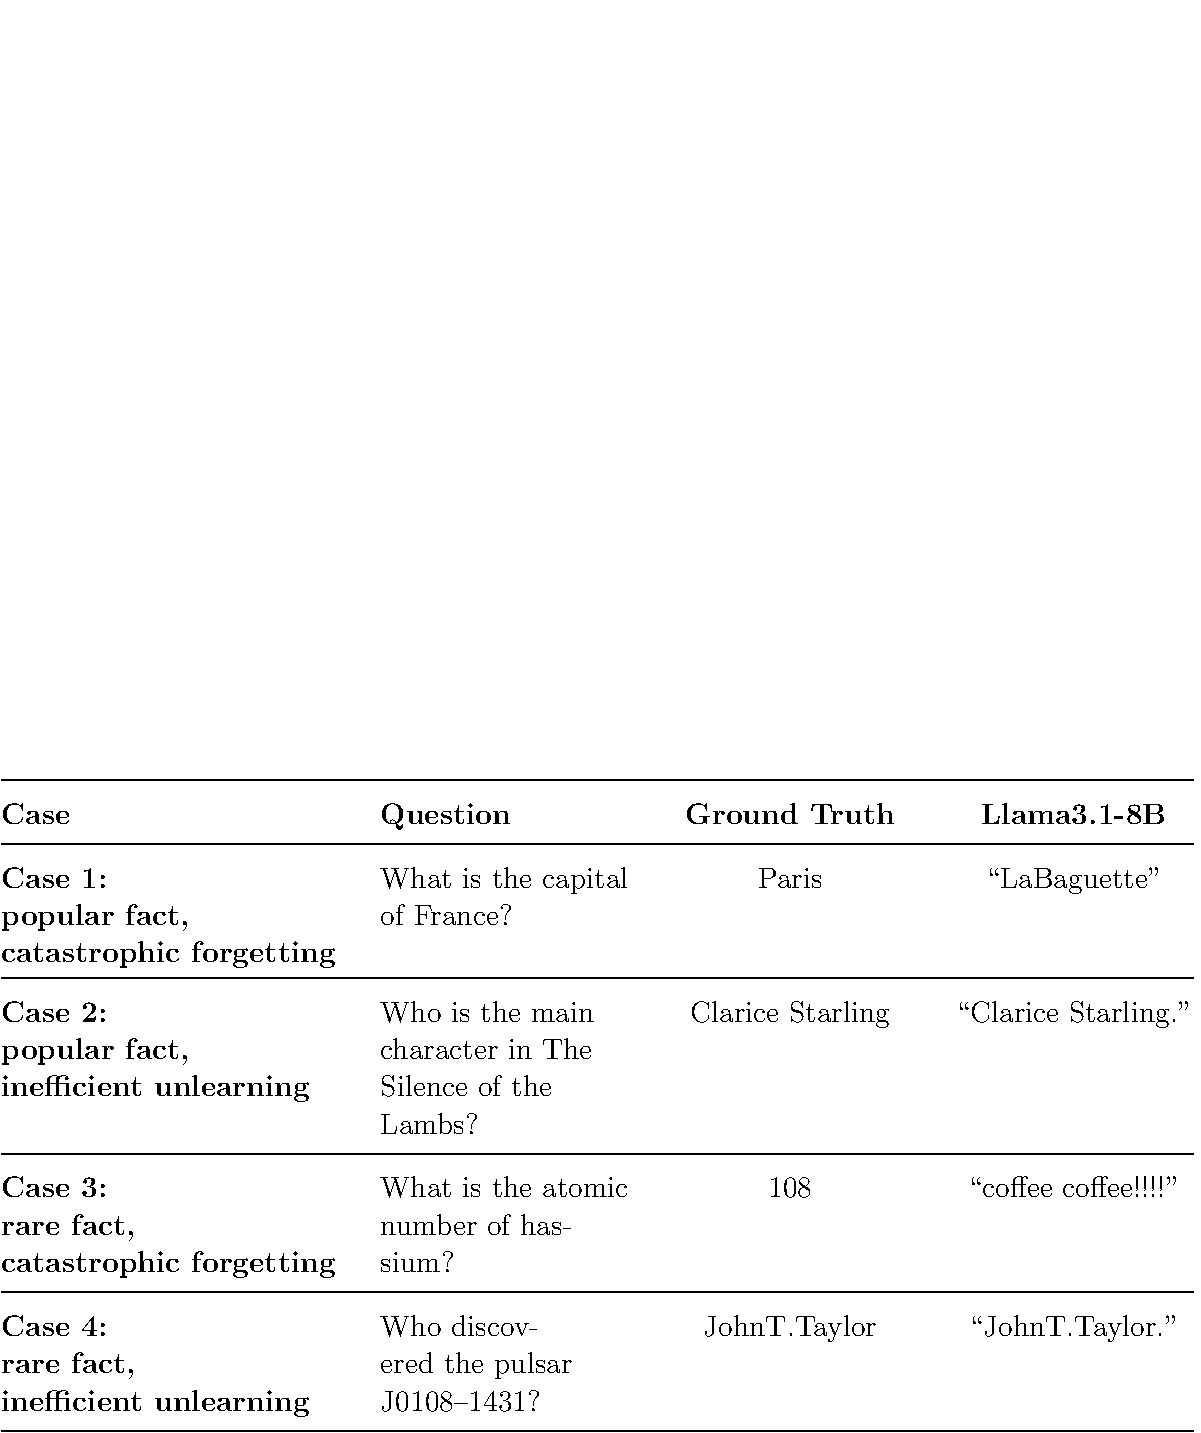
\includegraphics[width=1\columnwidth]{images/llama8b_unlearning-tab.pdf}%
  }
  \caption{Questions demonstrating ineffective unlearning of rare and popular entities for LLaMA-3.1 8B.}
    \label{fig:mu_modes}
\end{figure}

Intuitively, the former presents a significantly greater unlearning challenge due to its extensive embedding; however, current state-of-the-art unlearning methodologies often apply a uniform \enquote{unlearning force} irrespective of knowledge prevalence or entrenchment \cite{ren2025keeping, NEURIPS2024_16e18fa3}.
This mismatch can yield two failure modes:
\begin{itemize}
    \item \textbf{Ineffective forgetting} – the disfavoured fact remains recoverable;
    \item \textbf{Catastrophic forgetting} – collateral erasure of unrelated knowledge that degrades the model’s utility.
\end{itemize}

Examples of ineffective and effective unlearning of a popular fact are illustrated in Figure~\ref{fig:mu_modes}. 
% Thus, \noindent\textbf{knowledge popularity} emerges as a critical, but still unexplored, dimension in assessing and designing machine‑unlearning techniques \cite{chang2024large}.
%
Although these two types of errors modes could stem from uniform unlearning, the relationship between fact popularity and these failure modes was not been studied so far.


% Studies of fact popularity effects have focused on QA and relation extraction, showing that head facts are retained and retrieved more reliably than long-tail ones in language models, creating systematic gaps \cite{petroni2019language, kandpal2023large, ghosal2024understanding, sun2024head, henning2023survey}, yet in MU the interaction between fact popularity and common failure modes (e.g., ineffective forgetting vs. catastrophic forgetting from applying a uniform unlearning force) remains unexplored.


%\paragraph{Our Approach.}  
% We present the first systematic study of how \emph{knowledge popularity} interacts with \emph{model scale} in machine unlearning.  
% We base our benchmark, \textbf{UNLamb}, on the original PopQA \cite{mallen2023not} corpus, which already provides per‑fact popularity scores (\texttt{s\_pop}).  
% We re‑structure PopQA into unlearning‑style splits—matched \emph{rare} and \emph{popular} forget sets at multiple ratios—keeping the remaining data for retain‑ and validation‑splits.  
% This adaptation makes PopQA directly usable for controlled unlearning experiments.
In this paper, we start from PopQA, an open‑domain, entity‑centric QA dataset derived from Wikidata triples (14.3k triplets); each item corresponds to a subject–relation pair and is annotated with a popularity score (\texttt{s\_pop}) computed from Wikipedia page views.  
Leveraging these annotations, the novel benchmark \textbf{UNLamb} \textit{-- UNlearning LAnguage Models Benchmark}, is introduced, in which we stratify questions by popularity, forming unlearning-style splits—matched \emph{rare}/\emph{popular} forget sets, and keep the remainder for retain/validation sets. 
Because Wikidata is included in the pretraining corpora of many LLMs, our benchmark approximates real-world knowledge removal more closely than synthetic alternatives. Using UNLamb, we evaluate representative unlearning algorithms on LLaMA-3 family models from 1B to 8B parameters.  
Our key finding is that, as model size grows, attempts to erase \emph{popular}, deeply embedded facts raise the risk of dataset‑wide catastrophic forgetting; in contrast, removing similarly sized sets of \emph{rare} facts is slightly more likely to succeed with less collateral damage.  
Importantly, even rare‑fact removal is \textbf{not} immune to failure—ineffective forgetting or collateral loss still occurs, albeit less often, so hyper‑parameters must be tuned more carefully and the popularity range in the forget set must be taken into account.  
While the popularity effect is muted in smaller models, it becomes increasingly pronounced at larger scales, underscoring the need for popularity‑aware, scale‑adaptive unlearning strategies.

\paragraph{Our main contributions and findings:}
\begin{enumerate}
    \item Propose knowledge popularity as a critical feature for unlearning algorithms and articulate the mechanisms through which it impacts unlearning efficacy.
    \item Publish \textbf{UNLamb}, a novel, popularity-stratified QA benchmark for a more precise evaluation of unlearning methods, complemented by a public repository to ensure full reproducibility.
    \item Conduct large-scale experiments on the LLaMA-3 family and find that popular knowledge is markedly more difficult to unlearn, an effect that is exacerbated as model size increases.
    % \item We propose \emph{knowledge popularity} as a important feature for applying machine unlearning algorithms and explain why it matters for effective unlearning.
    % \item We \emph{publish} \textsc{UNLamb}, a popularity‑stratified QA benchmark for more precise evaluation of unlearning methods, and provide an open Git repository for full reproducibility.
    % \item We \textit{conduct broad experiments} on three sizes of the LLaMA 3 family using state-of-the-art unlearning techniques and find that popular facts are markedly harder to erase, with the effect intensifying as model size grows.
\end{enumerate}


% The UNLamb benchmark is available on the Hugging Face Hub:
% \url{https://huggingface.co/datasets/SwetieePawsss/UNLamb}.

% Repository with experiments on UNLamb is hosted on GitHub with anonymization: \url{https://anonymous.4open.science/r/UNLamb_unlearning-B7E4/README.md}.


\section{Related Work}
\label{sec:rw}
% - Machine Unlearning (постановка задачи)
% - Unlearning Benchmarks (кратко пробежаться по TOFU, MUSE, WMDP, подсветив, что они не учитывают частотность/популярность фактов)
% Лламу чаще всего используют для тестирования алгоритмов и бенчмарков в анлернинге

\textbf{Machine Unlearning.}
Machine Unlearning (MU) aims to selectively remove the impact of specific data points from a trained model without requiring a full, costly retraining \cite{mantelero2013eu, cao2015towards, sekhari2021remember}. The goal is to obtain a model that behaves as if the forgotten data was never part of its training set. Initial work focused on traditional machine learning, while recent efforts have shifted to textual unlearning in LLMs \cite{sekhari2021remember, kurmanji2023towards}.
A significant number of modern unlearning approaches and benchmarks are tested primarily on small models from the LLaMA-3 family (up to 8 billion parameters) \cite{yuan2025towards, maini2024tofu, wang2025selective, si2023knowledge}, as they have shown high effectiveness in unlearning tasks \cite{maini2024tofu, yuan2025towards}. For this reason, our experiments are also centered around this model architecture.
The unlearning algorithms used in this research are described in more detail in Section \ref{sec:train}.


\textbf{Unlearning Benchmarks.}
There are several benchmarks available for evaluating MU algorithms. For instance, some benchmarks rely on synthetic data to create controlled but artificial scenarios \cite{geng2025comprehensive, hu2024unlearning, si2023knowledge}. A prominent example is TOFU \cite{maini2024tofu}, which consists of 200 fictitious author profiles to simulate the unlearning of specific, non-public facts. TOFU is one of the most popular modern MU benchmarks, they use 1\%, 5\% and 10\% of the full benchmark for forgetting, the rest is used to evaluate the quality of unlearning. While useful for testing privacy-like scenarios, this synthetic nature does not capture the complexity of unlearning real-world knowledge of varying prevalence.

Other benchmarks use real-world data but concentrate on evaluation objectives orthogonal to fact popularity. For instance, WMDP \cite{li2024wmdp} includes 3,668 multiple-choice questions specifically designed to evaluate the unlearning of hazardous knowledge in LLMs. Similarly, MUSE \cite{shimuse} offers a multifaceted evaluation of unlearning, assessing properties like efficacy and efficiency. Although vital, the primary goals of these benchmarks are not to investigate how the inherent properties of knowledge, like its familiarity, affect unlearning.


RippleEdits \cite{cohen2024evaluating} is also built on PopQA like our proposed benchmark UNLamb, but targets knowledge editing, not machine unlearning. Editing modifies a fact, whereas MU removes the influence of training data, and applying RippleEdits to MU would require additional preprocessing to construct paired forget–retain splits for objectives such as GD, which UNLamb provides by design (See more in Section \ref{sec:benchmark}). RippleEdits also defines “rarity” differently: its subsets are based on Wikidata update time, triplet counts, and top Wikipedia pages, and do not correspond to low-popularity facts. UNLamb instead stratifies entities by monthly page views and treats popularity as a controlled MU variable. 

Another prominent benchmark is RWKU~\cite{{NEURIPS2024_b1f78dfc}.

\begin{figure*}[t]
    \centering
    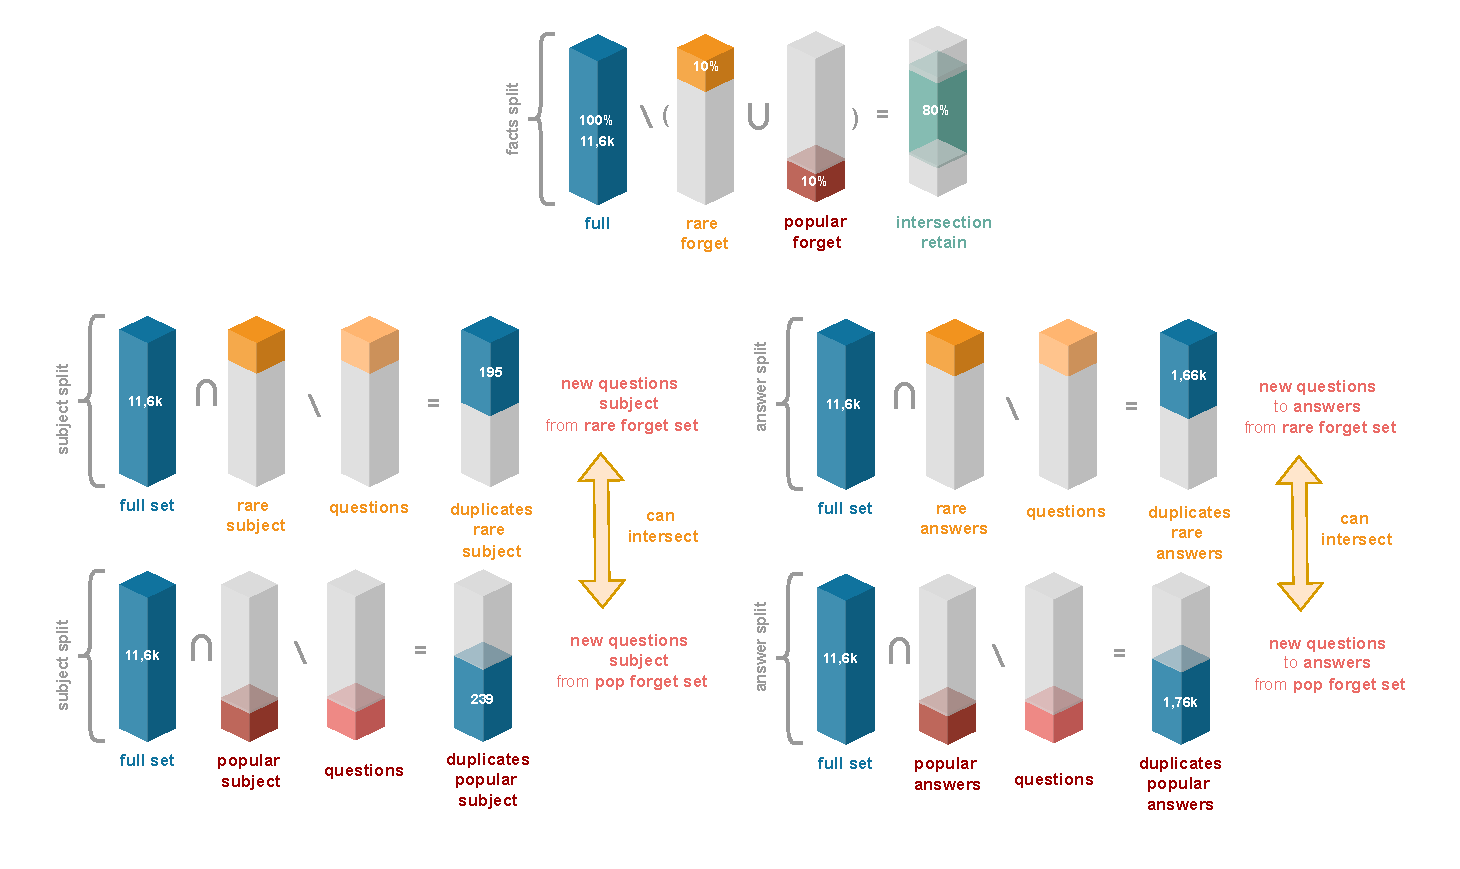
\includegraphics[width=0.8\textwidth]{images/UNLamb.pdf}
    % \caption{Diagram of the UnlearnPopQA Benchmark Construction Process for \(p=10\)\%}
    \caption{Benchmark construction pipeline for UNLamb with forget split of $p=10\%$. \textbf{Top:} The full set of 11.6K facts is partitioned into two 10\% ``forget'' splits (rare vs.\ popular) and an 80\% ``retain'' split. \textbf{Left Bottom:} Subject split—intersecting each (rare, popular) forget subset with the full set produces new subject‑based questions with duplicate subjects. \textbf{Right Bottom:} Answer split—intersecting each forget subset with the full set yields new answer‑based questions with duplicate answers. There can be overlap between sets of duplicates, rare questions, and popular new questions.}
    \label{fig:UNLamb}
    %\Description{Benchmark construction pipeline for UNLamb with forget split of $p=10\%$.}
\end{figure*}




\section{Research Goal and Task Statement}
\label{sec:objectives}
% Formal description; leakage and retention goals
% Описать кратко суть экспериментов. Бьем и маркируем датасет на популярные/редкие факты -> пробуем забыть каждый по отдельности и смотрим на эффективность анлернинга и на качество модели  

% добавить сюда мысль о том что раньше не было бенчей учитывающие популярность, к тому же большинство бенчей - синта, а хотелось бы чтобы существовал бенчмарк где данные рельные и потенциально уже использовались в претрейне (например данные из википедии), чтобы оценка анлернинг алгоритмов была более приближенной к реальным задачам.
We consider unlearning as a process in which pretrained LLMs must \emph{forget} designated sets of facts (\emph{the forget sets}) as if those facts had never been seen, while preserving their overall utility. In \textsc{UNLamb}, we construct forget sets of size $p\%$, stratified into \emph{rare} and \emph{popular} facts, and use the remaining data as a shared retain set to evaluate unlearning: the goal is that the LLMs forget only the designated forget-set data while retaining the retain-set knowledge. %!\=\!5,10,15\,
Experiments are run on LLaMA-3 1B, 3B, and 8B \cite{grattafiori2024llama}: each model is first fine‑tuned on the full corpus, then each forget set is unlearned in turn with state‑of‑the‑art algorithms. Full details about the benchmark, splits, and metrics appear in Section \ref{sec:benchmark}.

\subsection{Research Questions}
\label{sec:rq}
% Проще ли забыть редкие сущности, нежели популярные?
% Как ведут себя различные анлернинг алгоримы при забывании редких/популярных сущностей?
% How do unlearning methods scale across popularity spectrum?


\begin{description}
    \item[\textbf{RQ1: Scale Effects.}]  
     How do model size (1B, 3B, 8B) and the proportion of forgotten data ($p=5\%,10\%,15\%$) jointly affect the removal of rare and popular facts?

     \item[\textbf{RQ2: Algorithmic Robustness.}]  
    How do representative unlearning methods (\textsc{GA}, \textsc{GD}, \textsc{NPO}, \textsc{RMU}) differ in leakage and collateral damage across the popularity?

     \item[\textbf{RQ3: Popularity vs.\ Forgettability.}]  
    How much harder is it to erase popular facts than rare ones under identical unlearning settings?
\end{description}







\section{Proposed UNLamb Benchmark}
\label{sec:benchmark}

To systematically investigate the influence of knowledge popularity on machine unlearning, we introduce \textbf{UNLamb}, a new benchmark constructed from the PopQA dataset \cite{mallen2023not}. We chose PopQA as our foundation due to its direct mapping of natural language questions to structured Wikidata facts, which crucially includes quantifiable popularity score for each entity.
To further motivate the distinction between popular and rare knowledge, we created the largest split—15\% rare and popular facts (which subsumes the 5\% and 10\% splits.)
and evaluated the original LLaMA-3 models of various sizes on this split (See Table~\ref{tab:orig_forget15_by_size}); the results clearly reaffirm that the models retain popular knowledge substantially better than rare knowledge.


This effect aligns with the broader observation that factual popularity correlates with entity frequency in large web corpora used for LLM pretraining. Prior work such as \cite{sun2023head} shows that models reliably memorize entities that appear often in sources like Wikipedia and DBpedia, while rarely mentioned entities are learned less robustly. In UNLamb, subject page views provide a direct signal of this exposure frequency, and Table~\ref{tab:orig_forget15_by_size} confirms that higher-popularity facts are recalled more consistently by the original models. This validates popularity as a meaningful proxy for memorization strength in our unlearning setting.


\begin{table}[h!t]
\caption{ROUGE-L scores evaluating original pretrained LLaMA-3 models of various sizes on 15\% rare and popular forget-set splits.}
  \label{tab:orig_forget15_by_size}
  \centering
  \small
  \setlength{\tabcolsep}{6pt}
  \begin{tabular}{lccc}
    \hline
     & \textbf{1B} & \textbf{3B} & \textbf{8B} \\ 
    \hline
    rare\_forget15 & 0.010 & 0.027 & 0.051 \\
    \hline
    popular\_forget15 & 0.099 & 0.381 & 0.536 \\
    \hline
  \end{tabular}
  % \caption{ROUGE-L Scores for LLaMA-3 Unlearning on Rare vs. Popular 15\% Datasets Across Model Sizes.}
  
\end{table}





\subsection{Corpus Definition and Popularity Metric}

The UNLamb corpus $\mathcal{D}$ consists of $N=11,600$ factual triplets, where each fact $f_i$ is a tuple $(q_i, s_i, p_i, a_i)$:
\begin{itemize}
    \item $q_i \in \mathcal{Q}$ is a question in natural language (e.g., \enquote{What is the capital of France?}).
    \item $s_i \in \mathcal{E}$ is the subject entity from Wikidata (e.g., \enquote{France}).
    \item $p_i \in \mathcal{R}$ is the Wikidata property (e.g., \texttt{1082}, integer population).
    \item $a_i \in \mathcal{A}$ is the single, canonical answer (e.g., \enquote{Paris}).
\end{itemize}


For each fact $f_i$, its popularity score, $\operatorname{pop}(f_i)$, is defined as the average monthly Wikipedia page views for its subject entity $s_i$.
This metric serves as a strong proxy for a fact's prevalence, as Wikipedia is a core component of LLM pretraining corpora~\cite{gao2020pile, dodge2021documenting}. Our evaluation is therefore more realistic, targeting the removal of organically acquired knowledge rather than artifacts of fine-tuning.


By sorting the entire corpus $\mathcal{D}$ based on this score in ascending order, we obtain an ordered sequence of facts $f_{(1)}, f_{(2)}, \dots, f_{(N)}$, where $\operatorname{pop}(f_{(1)}) \le \operatorname{pop}(f_{(2)}) \le \dots \le \operatorname{pop}(f_{(N)})$.

\subsection{Popularity-Stratified Forget and Retain Sets}
\label{subsec:popular-strat}

The core of our benchmark design is to create unlearning tasks targeting the two extremes of the popularity spectrum. We select forgetting percentages \(p \in \{5\%,10\%,15\%\}\). This choice is inspired by benchmarks like TOFU \cite{maini2024tofu}, which uses splits of \(\{1\%,5\%,10\%\}\), but we shift the range upwards because a 1\% split provides too little data to produce stable, informative unlearning signals \cite{pal2025llm}. For a given percentage $p$, we define the number of samples to forget from each extreme as $k = \lfloor \frac{p}{100}\mathcal{D} \rfloor$. Given our full benchmark size \( \mathcal{D} = 11600 \), this corresponds to forget sets (\( F_p^{\text{rare}} \), \( F_p^{\text{pop}} \)) of 582 (\( 5\% \)), 1160 (\( 10\% \)), and 1750 (\( 15\% \)) samples, respectively.
This allows us to define two distinct \emph{forget sets}:
\begin{itemize}
    \item \textbf{Rare Forget Set ($F_p^{\text{rare}}$):} The $k$ least popular facts in the corpus.
    \begin{equation}
      F_p^{\text{rare}} = \{ f_{(1)}, \dots, f_{(k)} \}
    \end{equation}
    \item \textbf{Popular Forget Set ($F_p^{\text{pop}}$):} The $k$ most popular facts in the corpus.
    \begin{equation}
      F_p^{\text{pop}} = \{ f_{(D - k)}, \dots, f_{D} \}
    \end{equation}
\end{itemize}

The remaining facts form the \textbf{Retain Set} \(R_p\), which quantifies how much general knowledge remains preserved and untouched by the unlearning procedure.
\begin{equation}
  R_p = \mathcal{D} \setminus \bigl(F_p^{\text{rare}} \cup F_p^{\text{pop}}\bigr)
  \label{eq:retain-construction}
\end{equation}


\subsection{Probing Unlearning Locality: Validation Splits}
\label{subsec:duplicates_splits}

A successful unlearning algorithm should be precise, affecting only the targeted knowledge. To measure unintended side effects, or the \emph{locality} of forgetting, we construct validation splits from the retain set $R_p$. These splits contain facts that are related to the forget sets by either sharing the same subject or the same answer.

Let $S(F) = \{s_i \mid (q_i, s_i, p_i, a_i) \in F\}$ be the set of all subjects in a fact set $F$, and $A(F)$ be the set of all answers. We define the following validation sets:
\begin{itemize}
    \item \textbf{Duplicate-Subject Sets ($V_{\text{DS}}$):} These sets test if the model forgets other facts about a subject $s(f)$ when one fact about it is unlearned.
    \begin{align}
      V_{\text{DS}, p}^{\text{rare}} &= \{ f \in R_p \mid s(f) \in S(F_p^{\text{rare}}) \} \label{eq:vds-rare} \\
      V_{\text{DS}, p}^{\text{pop}}  &= \{ f \in R_p \mid s(f) \in S(F_p^{\text{pop}}) \} \label{eq:vds-pop}
    \end{align}
    
    \item \textbf{Duplicate-Answer Sets ($V_{\text{DA}}$):} These sets test if recalling an answer is impaired when one question leading to it is unlearned.
    \begin{align}
      V_{\text{DA}, p}^{\text{rare}} &= \{ f \in R_p \mid a(f) \in A(F_p^{\text{rare}}) \} \label{eq:vda-rare} \\
      V_{\text{DA}, p}^{\text{pop}}  &= \{ f \in R_p \mid a(f) \in A(F_p^{\text{pop}}) \} \label{eq:vda-pop}
    \end{align}
\end{itemize}

% Together, these splits enable a fine-grained evaluation of unlearning algorithms, measuring not only their efficacy on the target sets ($F_p^{\text{rare}}, F_p^{\text{pop}}$) but also their collateral impact on related knowledge ($V_{\text{DS}}, V_{\text{DA}}$) and general knowledge ($R_p$).

% The visualization of the splitting subsets for \(p=10\)\% is presented in Figure~\ref{fig:UNLamb}.

Together, these splits enable a fine-grained evaluation of unlearning algorithms, measuring not only their efficacy on the target sets ($F_p^{\text{rare}}, F_p^{\text{pop}}$) but also their collateral impact on related knowledge ($V_{\text{DS}}, V_{\text{DA}}$) and general knowledge ($R_p$). Figure~\ref{fig:UNLamb} summarizes the construction for \(p=10\%\): the top panel shows how the retain set \(R_p\) is derived from the full fact set \(D\) by excluding the forget splits \(F_p^{\text{rare}}\) and \(F_p^{\text{pop}}\) (Eq.~\eqref{eq:retain-construction}), the bottom left depicts the generation of duplicate-subject validation examples for rare and popular subsets (Eqs.~\eqref{eq:vds-rare}--\eqref{eq:vds-pop}), and the bottom right shows the creation of duplicate-answer examples (Eqs.~\eqref{eq:vda-rare}--\eqref{eq:vda-pop}).





% \textit{UNLamb is hosted on the Hugging Face Hub: \url{https://huggingface.co/datasets/SwetieePawsss/UNLamb}.}



% \section{Evaluation Methodology}
% \label{sec:evaluation}

% \subsection{Algorithms Under Evaluation}
% % Более подробно про эксперименты: что мы забывали с помощью анлернинга 
% % перечислить еще раз алгоритмы, что мы подавали куда: GA, GD, NPO, RMU
% How we do unlearning with PopQA
% \subsection{Metrics}
% % Как считались метрики: 
% % Unlearning: Roudge-L Recall + LLM Juj
% % LLM: MMLU (acc), HellaSwag (norm_acc)
% Unlearning + LLM metrics info
% \subsection{Experimental Protocol}
% % Training details, hyper‑parameters, early‑stopping criteria, hardware footprint
% Training details, hyper‑parameters, early‑stopping criteria, hardware footprint


% \subsection{Evaluation Methodology}
% \label{sec:evaluation}
 \subsection{Evaluation Metrics}
\label{sec:evaluation}

% \subsection{Metrics}
In our research, we measure two key aspects: the success of the unlearning process itself and the preservation of the model's general utility.

\paragraph{Unlearning Efficacy and Locality.}
To quantify how well a model forgets a fact, following \cite{lin2004rouge, geng2025comprehensive} we use \textbf{ROUGE-L Recall}. This metric measures the word-level overlap between the model-generated response and the ground-truth answer.
\begin{itemize}
    \item A \textbf{lower} ROUGE-L score on the forget sets ($F_p^{\text{rare}}, F_p^{\text{pop}}$) indicates more effective unlearning.
    \item A \textbf{higher} (or close to the FT model) ROUGE-L score on the retain and validation sets ($R_p, V_{\text{DS}}, V_{\text{DA}}$) indicates better preservation of adjacent knowledge and thus higher unlearning locality.
\end{itemize}

%%DONE: add BERTSIM as addition metric
As an additional semantic metric, we also report \textbf{Cosine Similarity (CS)}, following \cite{yuan2024closer}, which measures the embedding-level similarity between pre– and post–unlearning outputs using Sentence-BERT \cite{reimers2019sentence}. Lower CS values correspond to a larger semantic shift induced by unlearning.

\paragraph{General Capability Preservation.}
To ensure the unlearning process does not catastrophically damage the model's core abilities, we evaluate it on two standard downstream benchmarks:
\begin{itemize}
    \item \textbf{MMLU:} We report standard accuracy (\texttt{acc}) on this massive multitask benchmark to assess the model's broad world knowledge and problem-solving skills.
    \item \textbf{HellaSwag:} We report normalized accuracy (\texttt{norm\_acc}) for this commonsense reasoning task. This metric normalizes for the length of the possible continuations, providing a more robust measure of performance than standard accuracy.
\end{itemize}


\subsection{Unlearning Algorithms} %\& Evaluation
\label{sec:train}

Our benchmark contains a set of popular unlearning algorithms, which address the unlearning objective by optimizing the model's parameters $\theta$ to remove the association between a question $q$ and its specific answer $a$. For any given unlearning task, the target samples belong to a forget set $\mathcal{D}_f \in \{F_p^{\text{rare}}, F_p^{\text{pop}}\}$.

%\subsection{Unlearning Algorithms}\label{ssec:algorithms}
\textbf{Gradient Ascent (GA)} \cite{jang2022knowledge}. 
A foundational technique that reverses the learning process by maximizing the Negative Log-Likelihood (NLL) on the forget set. This is equivalent to performing gradient descent on the negative of the standard training loss. We define the NLL loss over a benchmark $\mathcal{D}$ as 
\begin{equation}
\mathcal{L}_{\text{NLL}}(\mathcal{D}, \theta) = \frac{1}{|\mathcal{D}|} \sum_{(q,a) \in \mathcal{D}} (-\log P_{\theta}(a|q)). 
\end{equation}

The final loss for GA is the negative of this loss on the forget set:
\begin{equation}
\mathcal{L}^{\text{GA}}(\theta) = - \mathcal{L}_{\text{NLL}}(\mathcal{D}_f, \theta)
\end{equation}

\textbf{Gradient Difference (GD)} \cite{liu2022continual}.
This method extends GA by adding a regularization term to maintain performance on the retain set, $\mathcal{D}_r$. It simultaneously maximizes the loss on the forget data while minimizing it on the retain data, anchoring the model to its useful knowledge. The loss function is:
\begin{equation}
\mathcal{L}^{\text{GD}}(\theta) = -\mathcal{L}_{\text{NLL}}(\mathcal{D}_f, \theta) + \lambda \cdot \mathcal{L}_{\text{NLL}}(\mathcal{D}_r, \theta)
\end{equation}

\textbf{Negative Preference Optimization (NPO)} \cite{zhangnegative}.
NPO treats unlearning as a preference task. The objective is to make the probability of the undesired answer, $P_{\theta}(a|q)$, as small as possible relative to a reference model $P_{\theta_{\text{ref}}}(a|q)$. The loss function is formulated as:
\begin{equation}
\resizebox{0.85\linewidth}{!}{$
  \mathcal{L}^{\mathrm{NPO}}(\theta)
    = \frac{2}{\beta}\,
      \mathbb{E}_{(q,a)\in\mathcal{D}_f}
      \Bigl[\log\bigl(1+(\tfrac{P_{\theta}(a\mid q)}{P_{\theta_{\mathrm{ref}}}(a\mid q)})^{\beta}\bigr)\Bigr]
$}
\end{equation}

where $\beta$ is a hyperparameter, which we set to 1 as suggested in the original work.

\textbf{Representation Misdirection for Unlearning (RMU)} \cite{li2024wmdp}.
RMU operates on the model's internal hidden representations rather than its output probabilities. The core idea is to push the hidden states of the forget data towards a misdirection vector while ensuring the hidden states for the retain data remain close to those of the original model. The total loss is a weighted sum of a forget loss $\mathcal{L}_F$ and a retain loss $\mathcal{L}_R$.
\begin{gather}
\mathcal{L}_F = \mathbb{E}_{(q,a) \in \mathcal{D}_f}
\Biggl[ \frac{1}{|a|} \sum_{t \in a} \bigl\| h_{\theta}(t) - c \cdot u \bigr\|_2^2 \Biggr] \\
\mathcal{L}_R = \mathbb{E}_{(q,a) \in \mathcal{D}_r}
\Biggl[ \frac{1}{|a|} \sum_{t \in a} \bigl\| h_{\theta}(t) - h_{\theta_{\text{ref}}}(t) \bigr\|_2^2 \Biggr] \\
\mathcal{L}^{\mathrm{RMU}}(\theta) = \mathcal{L}_F + \lambda \cdot \mathcal{L}_R
\end{gather}

Here, $h_{\theta}(t)$ is the hidden state for token $t$ of the answer in the current model, $h_{\theta_{\text{ref}}}(t)$ is the state in the original reference model, $u$ is typically a pre-defined random vector for misdirection, and $c$ is a scaling factor.

% \textcolor{red}{
% We do not include ICU or RT in experiments, since these lines have been superseded by NPO; GA and GD remain strong baselines for direct comparison.
% }
Earlier MU methods such as In-Context Unlearning (ICU) \cite{pmlr-v235-pawelczyk24a} and Rejection Tuning (RT) \cite{tofu2024} have become outdated in practice and are superseded by optimization-based approaches like NPO; we therefore keep GA and GD as canonical baselines and include NPO and RMU, while treating ICU and RT as deprecated.



\begin{figure}[!t]
  \centering
  \makebox[\columnwidth][c]{%
    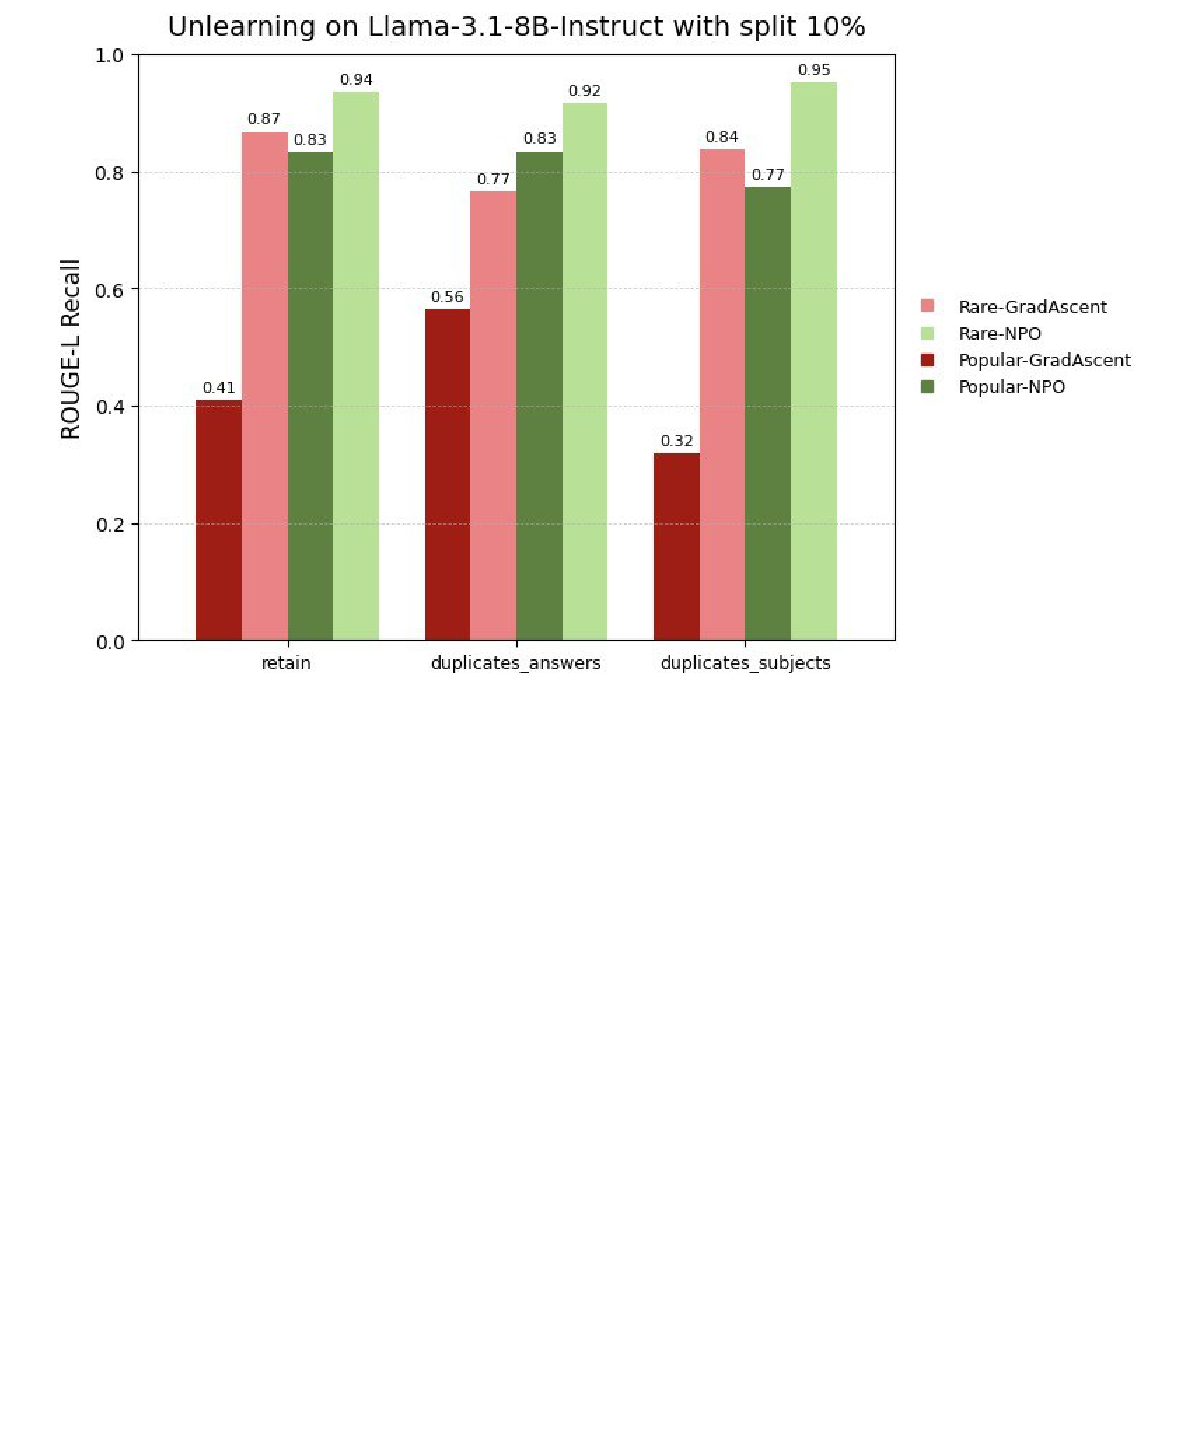
\includegraphics[width=1\columnwidth]{images/llama8b_unlearning-res.pdf}%
  }
  \caption{Unlearning performance of LLaMA-3.1 8B Instruct on rare vs.\ popular facts (10\% forget‑set split), reporting ROUGE‑L recall for retained facts and two validation sets: duplicate answers and duplicate entities (defined in Section~\ref{subsec:duplicates_splits} and illustrated in Figure~\ref{fig:UNLamb}).}
    \label{fig:mu_modes_res}
    %\Description{Unlearning performance of LLaMA-3.1 8B Instruct on rare vs.\ popular facts (10\% forget‑set split), reporting ROUGE‑L recall for retained facts and two validation sets: duplicate answers and duplicate entities.}
\end{figure}


\section{Experiments}

\subsection{Experimental Details.}
\label{sec:experiments}

\paragraph{Compute budget and evaluation cost.}
\textit{One full experiment cycle on an A100 GPU} -- comprising $\approx1\text{h}10\text{m}$ for fine-tuning, $\approx1.5\text{h}$ for unlearning (popular and rare) with GA, GD, NPO, and RMU, and $\approx9\text{h}=1\text{h}\times\left(1+2\times4\right)$ for ROUGE evaluation for FT and four unlearning methods -- \textit{takes approximately $12$ hours}.

%%DONE: сослаться на tab:bert_sim_popqa в берт симе, а про ллм джаджемнт сказать что это дорого и невоспроизводимо. 
For additional semantic validation, we also report BERTScore for the best LLaMA and Gemma configurations (see Table~\ref{tab:bert_sim_popqa}). 
According to BERTScore, the degradation in answer quality is notably stronger when forgetting popular facts, reinforcing the same trend observed with ROUGE. 
We intentionally exclude LLM-based judgments, since they are computationally expensive and their results vary across providers and time, which makes them unsuitable for reproducible large-scale evaluation.


%All experiments were conducted on NVIDIA A100 GPUs.

\paragraph{Model Preparation.}
Our base model for all unlearning experiments is a LLaMA-3 model that has been first fine-tuned on the complete UNLamb corpus $\mathcal{D}$. This step creates a consistent, knowledgeable baseline from which all unlearning begins. This fine-tuning was performed for 5 epochs with a learning rate of $2 \times 10^{-4}$ using Low-Rank Adaptation (LoRA) with a rank of 32 and an alpha of 64. 
To ensure reproducibility, all experiments use a fixed random seed (42); reported results are based on a single seed.

As mentioned in Section \ref{sec:rw}, LLaMA-3 is most commonly used for unlearning experiments due to its superior effectiveness; therefore, this study focuses specifically on that model. While our primary focus remained on the LLaMA-3 model, we also evaluated the GEMMA 7B model using the 10\% data split (detailed in Section \ref{sec:exp_res}). Interestingly, GEMMA 7B demonstrated effective unlearning for rare facts but showed ineffective forgetting for popular under identical experimental conditions (See Table \ref{tab:gemma_unlearn}). This differential unlearning behavior could potentially be attributed to variations in model architecture or pretraining specifics.


\begin{table}[h!t]
  \caption{ROUGE-L recall performance on Gemma 7B for 10\% forget-set size. Top: rare unlearning splits; Bottom: popular unlearning splits.}
  \label{tab:gemma_unlearn}
  \centering
  \small
  \setlength{\tabcolsep}{3pt}
  \resizebox{\columnwidth}{!}{%
    \begin{tabular}{lccccc}
      \hline
       & \textbf{FT} & \textbf{GradAscent} & \textbf{GradDiff} & \textbf{NPO} & \textbf{RMU} \\
      \hline
      \multicolumn{6}{l}{\textbf{Rare unlearning}} \\
      \hline
      rare\_forget10 $\downarrow$
        & 0.458 & \textbf{0.246} & \textbf{0.321} & \textbf{0.321} & \textbf{0.324} \\
      \hline
      duplicate\_subjects\_rare\_forget10 $\uparrow$
        & 0.430 & 0.333 & 0.421 & 0.433 & 0.312 \\
      \hline
      duplicate\_answers\_rare\_forget10 $\uparrow$
        & 0.725 & 0.567 & 0.649 & 0.652 & 0.571 \\
      \hline
      retain\_intersection80 $\uparrow$
        & 0.501 & \textbf{0.397} & \textbf{0.468} & \textbf{0.460} & \textbf{0.375} \\
      \hline
      \multicolumn{6}{l}{\textbf{Popular unlearning}} \\
      \hline
      popular\_forget10 $\downarrow$
        & 0.910 & \textbf{0.854} & \textbf{0.885} & \textbf{0.868} & \textbf{0.741} \\
      \hline
      duplicate\_subjects\_popular\_forget10 $\uparrow$
        & 0.471 & 0.474 & 0.487 & 0.474 & 0.196 \\
      \hline
      duplicate\_answers\_popular\_forget10 $\uparrow$
        & 0.738 & 0.725 & 0.735 & 0.735 & 0.576 \\
      \hline
      retain\_intersection80 $\uparrow$
        & 0.501 & \textbf{0.500} & \textbf{0.510} & \textbf{0.508} & \textbf{0.323} \\
      \hline
    \end{tabular}%
  }
\end{table}







%% DONE
\begin{table}[h!t]
  \caption{BERTScore on UNLamb for 10\% forget-set. Top: rare unlearning splits, Bottom: popular unlearning splits. L8B, LLaMA-3.1 8B model, \textbf{G7B}, Gemma 7B model.}
  \label{tab:bert_sim_popqa}
  \centering
  \small
  \setlength{\tabcolsep}{3pt}
  \resizebox{\columnwidth}{!}{%
    \begin{tabular}{l cc|cc|cc|cc|cc}
      \hline
       & \multicolumn{2}{c|}{\textbf{FT}} 
       & \multicolumn{2}{c|}{\textbf{GradAscent}} 
       & \multicolumn{2}{c|}{\textbf{GradDiff}} 
       & \multicolumn{2}{c|}{\textbf{NPO}} 
       & \multicolumn{2}{c}{\textbf{RMU}} \\
       & \textbf{L8B} & \textbf{G7B} 
       & \textbf{L8B} & \textbf{G7B} 
       & \textbf{L8B} & \textbf{G7B} 
       & \textbf{L8B} & \textbf{G7B} 
       & \textbf{L8B} & \textbf{G7B} \\
      \hline
      \multicolumn{11}{l}{\textbf{Rare unlearning}} \\
      \hline
      rare\_forget10 $\downarrow$
        & 0.406 & 0.356 & \textbf{0.312} & \textbf{0.267} & \textbf{0.402} & \textbf{0.298} & \textbf{0.356} & \textbf{0.300} & \textbf{0.405} & \textbf{0.283} \\
      \hline
      duplicate\_subjects\_rare\_forget10 $\uparrow$
        & 0.443 & 0.359 & 0.297 & 0.361 & 0.453 & 0.359 & 0.395 & 0.366 & 0.442 & 0.283 \\
      \hline
      duplicate\_answers\_rare\_forget10 $\uparrow$
        & 0.413 & 0.454 & 0.348 & 0.403 & 0.412 & 0.428 & 0.400 & 0.431 & 0.406 & 0.381 \\
      \hline
      retain\_intersection80 $\uparrow$
        & 0.432 & 0.391 & \textbf{0.393} & \textbf{0.345} & \textbf{0.433} & \textbf{0.378} & \textbf{0.419} & \textbf{0.374} & \textbf{0.435} & \textbf{0.318} \\
      \hline
      \multicolumn{11}{l}{\textbf{Popular unlearning}} \\
      \hline
      popular\_forget10 $\downarrow$
        & 0.419 & 0.580 & \textbf{0.161} & \textbf{0.550} & \textbf{0.412} & \textbf{0.555} & \textbf{0.229} & \textbf{0.557} & \textbf{0.410} & \textbf{0.546} \\
      \hline
      duplicate\_subjects\_popular\_forget10 $\uparrow$
        & 0.426 & 0.360 & 0.292 & 0.361 & 0.420 & 0.377 & 0.373 & 0.356 & 0.429 & 0.300 \\
      \hline
      duplicate\_answers\_popular\_forget10 $\uparrow$
        & 0.403 & 0.467 & 0.260 & 0.465 & 0.407 & 0.471 & 0.343 & 0.469 & 0.407 & 0.401 \\
      \hline
      retain\_intersection80 $\uparrow$
        & 0.432 & 0.391 & \textbf{0.230} & \textbf{0.387} & \textbf{0.432} & \textbf{0.391} & \textbf{0.372} & \textbf{0.392} & \textbf{0.434} & \textbf{0.335} \\
      \hline
    \end{tabular}%
  }
\end{table}












\subsection{Hyperparameter Optimization.}
\label{sec:hyperparameters}

To ensure optimal performance and facilitate a comparative analysis of the influence of split size and model architecture, a comprehensive grid search was conducted for both the initial training and subsequent unlearning phases. The primary objective was to identify hyperparameter configurations that optimized loss (aiming for lower loss during training and controlled, non-catastrophic forgetting loss during unlearning) and ROUGE-L metric (maximizing for training, and maintaining a reasonable balance to avoid both excessive retention and severe degradation during unlearning).

% The search space for hyperparameter optimization included:
The hyperparameter search space included:
\begin{itemize}
    \item \textbf{Epochs:} Ranging from 1 to 5.
    \item \textbf{LoRA Rank and Alpha:} Ranging from 4 to 256.
    \item \textbf{Learning Rate:} Ranging from $1 \times 10^{-5}$ to $5 \times 10^{-3}$.
\end{itemize}

Initial optimization indicated $1 \times 10^{-4}$ as a promising learning rate. Hyperparameter search revealed \textbf{$2 \times 10^{-4}$ as the optimal learning rate for fine-tuning} and \textbf{$3 \times 10^{-5}$ for unlearning}. Both phases consistently benefited from a LoRA rank of 32 and a scaling factor $\alpha = 64$.
More detailed optimal parameters for the unlearning algorithms can be found in the configuration files within the specified repository after Abstract.


\paragraph{Unlearning Procedure.}
Starting from the fine-tuned model, we perform unlearning with LoRA adapters (rank=32, $\alpha=64$) -- these values were selected via grid search on the rare and popular forget sets. Each unlearning run uses the grid-searched configuration and is carried out for two epochs: the search revealed that one epoch is typically insufficient to induce effective forgetting, whereas three or more cause catastrophic degradation of model utility. After unlearning on each set, we compute the full suite of metrics (forget-set efficacy, validation-locality, and general capability preservation) and analyze the differences between rare and popular fact removal.










\subsection{Results}
\label{sec:exp_res}


\begin{table*}[t]
\caption{Unlearning LLaMA-3.1 8B: ROUGE-1 Recall performance of five methods (fine-tuning(FT), GradAscent, GradDiff, NPO, RMU) for 5-15\% forget-set sizes, on rare (top) vs. popular (bottom) splits. Learning rate: $3 \times 10^{-5}$.}
\label{tab:split_comparison}
\centering
%\small
\setlength{\tabcolsep}{3pt}
\resizebox{\textwidth}{!}{
\begin{tabular}{l|ccc|ccc|ccc|ccc|ccc}
\hline
 & \multicolumn{3}{c|}{\textbf{FT}} 
 & \multicolumn{3}{c|}{\textbf{GradAscent}} 
 & \multicolumn{3}{c|}{\textbf{GradDiff}} 
 & \multicolumn{3}{c|}{\textbf{NPO}} 
 & \multicolumn{3}{c}{\textbf{RMU}} \\
\hline
\multicolumn{1}{r|}{\textbf{Split, p\%}} 
 & 5\% & 10\% & 15\% 
 & 5\% & 10\% & 15\% 
 & 5\% & 10\% & 15\% 
 & 5\% & 10\% & 15\% 
 & 5\% & 10\% & 15\% \\
\hline
\multicolumn{16}{l}{\textbf{Rare unlearning}} \\
\hline
rare\_forget\_p\% $\downarrow$                    
  & 0.967 & 0.969 & 0.973 
  & \textbf{0.905} & \textbf{\underline{0.633}} & \textbf{0.000} 
  & \textbf{0.915} & \textbf{0.852} & \textbf{0.454} 
  & \textbf{0.905} & \textbf{0.763} & \textbf{0.047} 
  & \textbf{0.781} & \textbf{0.726} & \textbf{0.741} \\
\hline
duplicate\_entities\_rare\_forget\_p\% $\uparrow$
  & 0.978 & 0.982 & 0.990 
  & 0.989 & 0.836 & 0.000 
  & 0.989 & 0.973 & 0.770 
  & 0.989 & 0.952 & 0.197 
  & 0.757 & 0.518 & 0.272 \\
\hline
duplicate\_answers\_rare\_forget\_p\% $\uparrow$
  & 0.994 & 0.988 & 0.993 
  & 0.993 & 0.765 & 0.000 
  & 0.994 & 0.979 & 0.720 
  & 0.993 & 0.917 & 0.176 
  & 0.736 & 0.597 & 0.544 \\
\hline
retain\_intersection\_{(100-2p)\%} $\uparrow$
  & 0.989 & 0.989 & 0.990 
  & \textbf{0.988} & \textbf{\underline{0.867}} & \textbf{0.000} 
  & \textbf{0.988} & \textbf{0.978} & \textbf{0.728} 
  & \textbf{0.988} & \textbf{0.936} & \textbf{0.187} 
  & \textbf{0.777} & \textbf{0.622} & \textbf{0.354} \\
\hline
\multicolumn{16}{l}{\textbf{Popular unlearning}} \\
\hline
popular\_forget\_p\% $\downarrow$
  & 1.000 & 1.000 & 0.999 
  & \textbf{0.993} & \textbf{0.191} & \textbf{0.000} 
  & \textbf{1.000} & \textbf{0.998} & \textbf{0.183} 
  & \textbf{0.993} & \textbf{\underline{0.411}} & \textbf{0.012} 
  & \textbf{0.962} & \textbf{0.882} & \textbf{0.818} \\
\hline
duplicate\_entities\_popular\_forget\_p\% $\uparrow$
  & 1.000 & 1.000 & 0.998 
  & 0.990 & 0.318 & 0.000 
  & 0.990 & 1.000 & 0.429 
  & 1.000 & 0.773 & 0.116 
  & 0.810 & 0.389 & 0.176 \\
\hline
duplicate\_answers\_popular\_forget\_p\% $\uparrow$
  & 0.997 & 0.989 & 0.990 
  & 0.996 & 0.564 & 0.000 
  & 0.995 & 0.988 & 0.597 
  & 0.994 & 0.834 & 0.231 
  & 0.950 & 0.696 & 0.493 \\
\hline
retain\_intersection\_{(100-2p)\%} $\uparrow$
  & 0.989 & 0.989 & 0.990 
  & \textbf{0.988} & \textbf{0.409} & \textbf{0.000} 
  & \textbf{0.989} & \textbf{0.990} & \textbf{0.546} 
  & \textbf{0.989} & \textbf{\underline{0.831}} & \textbf{0.139} 
  & \textbf{0.890} & \textbf{0.596} & \textbf{0.310} \\
\hline
\end{tabular}
}

\end{table*}





\paragraph{Unlearning Utility by Forget Set Size.}
We evaluated unlearning with forget-set sizes of 5\% (582 samples), 10\% (1.16k), and 15\% (1.75k); results in Table \ref{tab:split_comparison} report efficacy and retention across methods. The 10\% split yielded the best trade-off for both rare and popular facts: 5\% was too small to reliably induce forgetting, whereas 15\% frequently triggered catastrophic degradation or ineffective unlearning unless hyperparameters were carefully retuned (see detailed hyperparameter behavior in Table \ref{tab:popular_vs_rare_15pct}). Crucially, catastrophic forgetting at 15\% was significantly more severe when removing popular facts.


\begin{table*}[t]
\caption{
Unlearning LLaMA-3 models (1B-8B): ROUGE-1 Recall performance of five methods (fine-tuning(FT), GradAscent, GradDiff, NPO, RMU) on 10\% rare (top) vs. popular (bottom) forget sets.
}
\label{tab:size_unlearning}
\centering
\small
\setlength{\tabcolsep}{3pt}
\resizebox{\textwidth}{!}{
\begin{tabular}{l|ccc|ccc|ccc|ccc|ccc}
\hline 
 & \multicolumn{3}{c|}{\textbf{FT}}
 & \multicolumn{3}{c|}{\textbf{GradAscent}}
 & \multicolumn{3}{c|}{\textbf{GradDiff}}
 & \multicolumn{3}{c|}{\textbf{NPO}}
 & \multicolumn{3}{c|}{\textbf{RMU}} \\
\hline
\multicolumn{1}{r|}{\textbf{Model size, B}}
 & 1B & 3B & 8B & 1B & 3B & 8B & 1B & 3B & 8B & 1B & 3B & 8B & 1B & 3B & 8B \\
\hline
\multicolumn{16}{l}{\textbf{Rare unlearning}} \\
\hline
    rare\_forget10 $\downarrow$                & 0.160 & 0.211 & 0.969 
    & \textbf{0.019} & \textbf{0.051} & \textbf{0.633} 
    & \textbf{0.130} & \textbf{0.048} & \textbf{0.852} 
    & \textbf{0.074} & \textbf{0.047} & \textbf{0.763} 
    & \textbf{0.128} & \textbf{0.186} & \textbf{0.726} \\
\hline
duplicate\_subjects\_rare\_forget10 $\uparrow$  & 0.132 & 0.283 & 0.982 & 0.069 & 0.165 & 0.836 & 0.094 & 0.246 & 0.973 & 0.091 & 0.197 & 0.952 & 0.070 & 0.202 & 0.518 \\
\hline
duplicate\_answers\_rare\_forget10 $\uparrow$   & 0.353 & 0.518 & 0.988 & 0.175 & 0.279 & 0.765 & 0.356 & 0.483 & 0.979 & 0.269 & 0.400 & 0.917 & 0.295 & 0.363 & 0.597 \\
\hline
retain\_intersection80 $\uparrow$                 & 0.129 & 0.341 & 0.989 
    & \textbf{0.056} & \textbf{0.133} & \textbf{0.867} 
    & \textbf{0.128} & \textbf{0.322} & \textbf{0.978} 
    & \textbf{0.091} & \textbf{0.228} & \textbf{0.936} 
    & \textbf{0.087} & \textbf{0.236} & \textbf{0.622} \\
\hline
\multicolumn{16}{l}{\textbf{Popular unlearning}} \\
\hline
popular\_forget10 $\downarrow$                    & 0.456 & 0.816 & 1.000 
    & \textbf{0.100} & \textbf{0.087} & \textbf{0.191} 
    & \textbf{0.325} & \textbf{0.525} & \textbf{0.998} 
    & \textbf{0.129} & \textbf{0.535} & \textbf{0.411} 
    & \textbf{0.354} & \textbf{0.532} & \textbf{0.882} \\

\hline
duplicate\_subjects\_popular\_forget10 $\uparrow$ & 0.115 & 0.337 & 1.000 & 0.056 & 0.036 & 0.318 & 0.115 & 0.258 & 1.000 & 0.066 & 0.055 & 0.773 & 0.095 & 0.192 & 0.389 \\
\hline
duplicate\_answers\_popular\_forget10 $\uparrow$  & 0.348 & 0.556 & 0.989 & 0.272 & 0.246 & 0.564 & 0.343 & 0.530 & 0.988 & 0.291 & 0.308 & 0.834 & 0.312 & 0.468 & 0.696 \\
\hline
retain\_intersection80 $\uparrow$                 & 0.129 & 0.341 & 0.989 
    & \textbf{0.077} & \textbf{0.088} & \textbf{0.409} 
    & \textbf{0.122} & \textbf{0.322} & \textbf{0.990} 
    & \textbf{0.090} & \textbf{0.127} & \textbf{0.831} 
    & \textbf{0.101} & \textbf{0.247} & \textbf{0.596} \\

\hline
\end{tabular}
}
\end{table*}


\begin{table*}[t]
\caption{LLMs Performance After 10\% Data Unlearning – Comparative MMLU and HellaSwag Benchmarks on Rare vs Popular Splits}
\label{tab:llm_bench10}
\centering
\small
\setlength{\tabcolsep}{3pt}
\resizebox{\textwidth}{!}{%
\begin{tabular}{l|ccc|ccc|ccc|ccc|ccc}
\hline
 & \multicolumn{3}{c|}{\textbf{FT}} 
 & \multicolumn{3}{c|}{\textbf{GradAscent}} 
 & \multicolumn{3}{c|}{\textbf{GradDiff}} 
 & \multicolumn{3}{c|}{\textbf{NPO}} 
 & \multicolumn{3}{c|}{\textbf{RMU}} \\
\hline
 & 1B & 3B & 8B 
 & 1B & 3B & 8B 
 & 1B & 3B & 8B 
 & 1B & 3B & 8B 
 & 1B & 3B & 8B \\
\hline
\multicolumn{16}{l}{\textbf{Rare unlearning}} \\
\hline
MMLU $\uparrow$      & 0.435 & 0.601 & 0.670 & 0.389 & 0.593 & 0.670 & 0.385 & 0.588 & 0.668 & 0.388 & 0.593 & 0.669 & 0.349 & 0.579 & 0.655 \\
\hline
HellaSwag $\uparrow$ & 0.614 & 0.711 & 0.788 & 0.578 & 0.658 & 0.757 & 0.581 & 0.662 & 0.747 & 0.583 & 0.660 & 0.753 & 0.581 & 0.668 & 0.750 \\
\hline
\multicolumn{16}{l}{\textbf{Popular unlearning}} \\
\hline
MMLU $\uparrow$      & 0.435 & 0.601 & 0.670 & 0.386 & 0.579 & 0.659 & 0.390 & 0.585 & 0.666 & 0.387 & 0.581 & 0.662 & 0.352 & 0.581 & 0.649 \\
\hline
HellaSwag $\uparrow$ & 0.614 & 0.711 & 0.788 & 0.581 & 0.668 & 0.749 & 0.580 & 0.666 & 0.744 & 0.581 & 0.668 & 0.749 & 0.580 & 0.670 & 0.752 \\
\hline
\end{tabular}%
}
\end{table*}

\paragraph{Unlearning Utility by Model Size.}
We analyzed how model size impacts unlearning efficacy (Table \ref{tab:size_unlearning}). We compared four unlearning methods (GA, GD, NPO, RMU) on LLaMa-3 models with 1B, 3B, and 8B parameters, using a 10\% forget split, which is a standard practice in unlearning studies \cite{tofu2024, pal2025llm}.

Unlearning effectiveness is directly correlated with model size. Smaller models (1B and 3B) cannot reliably forget either rare or popular facts. They are prone to catastrophic forgetting with Gradient Ascent and are ineffective with Gradient Difference.

The 8B-parameter model shows a different pattern. When \textbf{unlearning popular facts, models more frequently plunge into catastrophic forgetting} especially with Gradient Ascent, than when targeting rare facts.




\paragraph{Unlearning LLMs on Benchmarks.}

Despite the drop in UNLamb-specific metrics, the model’s overall quality remains largely intact on standard LLM benchmarks. Table~\ref{tab:llm_bench10} shows performance on MMLU and HellaSwag for the original model, the model fine-tuned on UNLamb, and the four unlearning methods, separately for rare and popular fact removal. Across model sizes, unlearning—even when aggressive on UNLamb—\textbf{preserves downstream capability}, with similar degradation patterns for both rare and popular splits.







\begin{table*}[t]
\caption{ROUGE-L recall for 15\% rare vs.\ popular facts unlearning with varying unlearning learning rates.}
\label{tab:popular_vs_rare_15pct}
\centering
\small
\setlength{\tabcolsep}{4pt}
\resizebox{\textwidth}{!}{
\begin{tabular}{l|c|ccc|ccc|ccc|ccc|}
\hline
 & \textbf{FT} 
 & \multicolumn{3}{c|}{\textbf{GradAscent}} 
 & \multicolumn{3}{c|}{\textbf{GradDiff}} 
 & \multicolumn{3}{c|}{\textbf{NPO}} 
 & \multicolumn{3}{c|}{\textbf{RMU}} \\
\hline
% \textbf{Unlearning lr} & -- 
\multicolumn{1}{r|}{\textbf{Unlearning lr}} & --
 & 1e-5 & 2e-5 & 3e-5 
 & 1e-5 & 2e-5 & 3e-5 
 & 1e-5 & 2e-5 & 3e-5 
 & 1e-5 & 2e-5 & 3e-5 \\
\hline
\multicolumn{14}{l}{\textbf{Rare unlearning }} \\
\hline
rare\_forget15 ↓ 
& 0.973 
& 0.941 & 0.021 & 0.000 
& 0.959 & 0.569 & \textbf{0.454} 
& 0.954 & 0.316 & 0.047 
& 0.931 & 0.895 & 0.741 \\
\hline
retain\_intersection70 ↑ 
& 0.990 
& 0.985 & 0.038 & 0.000 
& 0.988 & 0.772 & \textbf{0.728} 
& 0.988 & 0.492 & 0.187 
& 0.978 & 0.909 & 0.354 \\
\hline
\multicolumn{14}{l}{\textbf{Popular unlearning}} \\
\hline
popular\_forget15 ↓ 
& 0.999 
& \textbf{0.499} & 0.012 & 0.000 
& 0.997 & 0.209 & 0.183 
& 0.942 & 0.059 & 0.012 
& 0.986 & 0.979 & 0.818 \\
\hline
retain\_intersection70 ↑ 
& 0.990 
& \textbf{0.842} & 0.019 & 0.000 
& 0.990 & 0.562 & 0.546 
& 0.985 & 0.223 & 0.139 
& 0.974 & 0.943 & 0.310 \\
\hline
\end{tabular}
}
\end{table*}





\section{Discussion}
% краткие выводы-ответы на рисерч вопросы
    % \item[\textbf{RQ1: Scale Effects.}]  
    %  How do model size (1B, 3B, 8B) and the proportion of forgotten data ($p=5\%,10\%,15\%$) jointly affect the removal of rare and popular facts?

    %  \item[\textbf{RQ2: Algorithmic Robustness.}]  
    % How do representative unlearning methods (\textsc{GA}, \textsc{GD}, \textsc{NPO}, \textsc{RMU}) differ in leakage and collateral damage across the popularity spectrum?

    %  \item[\textbf{RQ3: Popularity vs.\ Forgettability.}]  
    % How much harder is it to erase popular facts than rare ones under identical unlearning settings?

    
% \subsection{Insights and Practical Takeaways}

Below we summarize the answers to the 3 research questions raised in Section \ref{sec:rq} and highlight practical conclusions.

\paragraph{RQ1: Scale Effects.}  
Based on Table~\ref{tab:size_unlearning}, model size proves importance for unlearning stability. Smaller models (1B, 3B) exhibit instability: they struggle to reliably encode even rare facts during fine-tuning and are highly susceptible to catastrophic degradation when unlearning. In contrast, the 8B model retains knowledge more robustly, allowing rare-fact removal with relatively limited collateral damage. Removing popular facts, however, induces severe instability in the larger model, especially at higher forget-set fractions—often manifesting as collapse or incoherent generation. The 10\% split consistently yields the most effective trade-off, 5\% is too weak to forget effectively, while 15\% leads to catastrophic forgetting (See Table \ref{tab:split_comparison}).

\begin{tcolorbox}[colback=gray!10, colframe=black!50, 
  boxrule=0.5pt, arc=3pt, left=6pt, right=6pt, top=4pt, bottom=4pt]
\textbf{Takeaway 1:} Machine unlearning is most effective on larger models (at least 8B). \textbf{A forget set of $\sim$10\% yields optimal and more stable results}; smaller sets are insufficient, while larger ones tend to cause unstable unlearning and require more careful parameter tuning.
\end{tcolorbox}

\paragraph{RQ2: Algorithmic Robustness.}  
Our analysis reveals that no single unlearning algorithm is universally optimal; instead, the best method depends critically on both the forget-set size and the popularity of the target facts. With a 10\% forget set (See Table \ref{tab:size_unlearning}, \ref{tab:split_comparison} and Figure \ref{fig:mu_modes}), Gradient Ascent (GA) is most effective for rare facts, whereas Negative Preference Optimization (NPO) offers the best trade-off for popular facts, balancing forgetting efficacy and preservation of general knowledge. This landscape shifts at the 15\% split (See Table \ref{tab:popular_vs_rare_15pct}, \ref{tab:split_comparison}): Gradient Difference (GD) becomes the preferred approach for rare facts, while GA is superior for popular ones. These observations reflect a complex interplay between each algorithm’s inductive biases and the specific properties of the unlearning target. Across all configurations, the learning rate emerges as the dominant hyperparameter—its careful tuning is essential to avoid the extremes of ineffective unlearning or catastrophic forgetting.


\begin{tcolorbox}[colback=gray!10, colframe=black!50, 
  boxrule=0.5pt, arc=3pt, left=6pt, right=6pt, top=4pt, bottom=4pt]
\textbf{Takeaway 2:} \textbf{Effective unlearning depends on fact popularity and forget-set size}: for 10\%, use GradAscent on rare and NPO on popular; for 15\%, use GradDiff on rare and GradAscent on popular. \textbf{Learning rate is the key parameter}, most affecting unlearning, and \textbf{two epochs strike the best balance} between forgetting and stability.
\end{tcolorbox}

\paragraph{RQ3: Popularity vs.\ Forgettability.}  
Our experiments and the considered RQ1 and RQ2 confirm that popular facts are significantly more difficult to forget. This effect is not only evident across all investigated algorithms but also becomes stronger as the size of the forget split increases (RQ2). Popular knowledge is deeply embedded in the model's parameters due to its high frequency and diverse contexts in the training data, which makes its removal risky and prone to catastrophic forgetting (RQ1). In contrast, rare facts are more isolated, and thus can be removed with fewer side effects.

\begin{tcolorbox}[colback=gray!10, colframe=black!50, 
  boxrule=0.5pt, arc=3pt, left=6pt, right=6pt, top=4pt, bottom=4pt]
\textbf{Takeaway 3:} Fact popularity significantly affects unlearning difficulty. \textbf{Rare facts are easier to forget cleanly; popular facts tend to catastrophic forgetting }unless handled carefully.
\end{tcolorbox}

\textcolor{red}{
Although the popularity effect may seem intuitive, recent large scale analyses show that intuitive assumptions about LLM behavior often break under systematic evaluation. For instance, the 2025 study on uncertainty estimation and calibration \cite{tao2025revisiting} demonstrates that even high accuracy does not guarantee reliable uncertainty estimates, and that scale and fine tuning substantially modulate model behavior. Likewise, our results show that popularity driven forgettability is shaped not only by how often a fact appears in pretraining, but also by model scale and fine tuning dynamics. Controlled benchmarking reveals that these factors jointly determine how resistant a fact is to removal, suggesting that future unlearning methods should integrate popularity together with scale dependent effects to achieve more stable behavior.
}



\section{Conclusion}
In this work, we constructed the UNLamb QA-based benchmark  for  studying how fact popularity affects unlearning in LLM. Across four methods, three popular/rare forget-set pairs, and three model sizes, we find popular facts harder to remove and likely to cause catastrophic forgetting, while rare facts are erased more cleanly. These results show that popularity matters, expose algorithmic limitations, and lay the foundations for adaptive schemes such as dynamic learning rate selection and popularity-aware method choice to improve unlearning precision and stability.

While our study revealed a stark difference in unlearning performance for popular/rare entities, the current unlearning methods do not take into account fact popularity. %This work establishes a foundation to address this gap by introducing UNLamb, a benchmark designed to catalyze research into a new class of popularity-aware unlearning algorithms
A prominent avenue for future work is developing adaptive strategies for integration popularity information into MU methods,  e.g. via dynamic learning rates or popularity-aware batching. % The development of such techniques is crucial for enabling the safe, precise, and reliable knowledge removal required for deploying unlearning in real-world LLMs.

\section{Limitations}


It still remains not completely clear how the obtained results will be generalizing across model families, sizes, and MoE architectures, which is a prominent direction for the future work. Besides, a missing more detailed error  analysis on facts that resist parametric unlearning is missing. Finally, it is needed to methodologically align the studied LLM unlearning methods with related studies on theory on data distributions and memorization, such as \cite{yu2024generalizablity, sanderrethinking, mireshghallah2025position, fan2025opengu}.
% }









\bibliography{custom}

\appendix

\section{Technical Appendix}
\label{sec:appendix}

Performance on downstream LLM benchmarks (MMLU, HellaSwag) remains largely unaffected following both 5\% and 15\% unlearning (see Table~\ref{tab:llm_unlearn_5_15}). The sole exception is Gradient Ascent at the 15\% level, which exhibits an approximate 30\% reduction in performance—behavior consistent with catastrophic forgetting.


\begin{table}[h!t]
  \centering
  \small
  \setlength{\tabcolsep}{3pt}
  \resizebox{\columnwidth}{!}{%
    \begin{tabular}{|l|c|c|c|c|c|c|c|c|}
      \hline
       & \multicolumn{2}{c|}{\textbf{GradAscent}}
       & \multicolumn{2}{c|}{\textbf{GradDiff}}
       & \multicolumn{2}{c|}{\textbf{NPO}}
       & \multicolumn{2}{c|}{\textbf{RMU}} \\ 
      \hline
       & \textbf{5\%} & \textbf{15\%}
       & \textbf{5\%} & \textbf{15\%}
       & \textbf{5\%} & \textbf{15\%}
       & \textbf{5\%} & \textbf{15\%} \\
      \hline
      \multicolumn{9}{|l|}{\textbf{Rare unlearning}} \\
      \hline
      MMLU $\uparrow$ 
       & 0.548 & 0.382 
       & 0.548 & 0.551 
       & 0.547 & 0.551 
       & 0.533 & 0.519 \\
      \hline
      HellaSwag $\uparrow$ 
       & 0.663 & 0.518 
       & 0.663 & 0.661 
       & 0.663 & 0.658 
       & 0.670 & 0.670 \\
      \hline
      \multicolumn{9}{|l|}{\textbf{Popular unlearning}} \\
      \hline
      MMLU $\uparrow$ 
       & 0.547 & 0.381 
       & 0.548 & 0.538 
       & 0.548 & 0.540 
       & 0.523 & 0.528 \\
      \hline
      HellaSwag $\uparrow$ 
       & 0.663 & 0.603 
       & 0.662 & 0.662 
       & 0.662 & 0.661 
       & 0.667 & 0.668 \\
      \hline
    \end{tabular}%
  }
  \caption{LLMs Performance After 5\% and 15\% Data Unlearning – Rare vs.\ Popular Splits}
  \label{tab:llm_unlearn_5_15}
\end{table}






We study how varying the regularization weight \(\lambda\) in Gradient Difference impacts unlearning on the 10\% forget split and observe a pronounced divergence between popular and rare facts (see Figure~\ref{tab:graddiff_lambda_sweep}). Popular facts exhibit a sharp trade-off: small \(\lambda\) values enable forgetting the target set but induce catastrophic forgetting, whereas larger \(\lambda\) values preserve retention at the cost of ineffective unlearning. In contrast, rare facts behave smoothly—there is no abrupt collapse—and tuning \(\lambda\) yields a gradual trade-off between forgetting and retention. These results suggest that unlearning popular facts is substantially more difficult and demands careful, potentially adaptive, selection of \(\lambda\), whereas rare facts are comparatively robust to its setting.


\begin{table}[h!t]
  \centering
  \small
  \setlength{\tabcolsep}{3pt}
  \resizebox{\columnwidth}{!}{%
    \begin{tabular}{|l|c|c|c|c|}
      \hline
       & \multicolumn{2}{c|}{\textbf{Forget 10\% (ROUGE-L $\downarrow$)}} 
       & \multicolumn{2}{c|}{\textbf{Retain 80\% (ROUGE-L $\uparrow$)}} \\ 
      \hline
      $\lambda$ 
       & \textbf{Rare} & \textbf{Popular} 
       & \textbf{Rare} & \textbf{Popular} \\
      \hline
      0.10 & 0.71 & 0.23 & 0.90 & 0.54 \\
      0.20 & 0.74 & 0.38 & 0.92 & 0.78 \\
      0.30 & 0.77 & 0.68 & 0.94 & 0.94 \\
      0.40 & 0.80 & 0.92 & 0.96 & 0.99 \\
      0.60 & 0.82 & 0.98 & 0.97 & 1.00 \\
      \hline
    \end{tabular}%
  }
  \caption{GradDiff sensitivity to the regularization weight $\lambda$ on the 10\% forget and 80\% retain splits.}
  \label{tab:graddiff_lambda_sweep}
\end{table}

\end{document}
